\subsection*{Aufgabe 8}
Das folgende S�ulendiagramm zeigt die Verteilung des Merkmals "Kinderzahl" f�r alle
Haushalte eines bestimmten Wohnviertels.
\begin{center}
\begin{figure}[!htbp]
\fbox{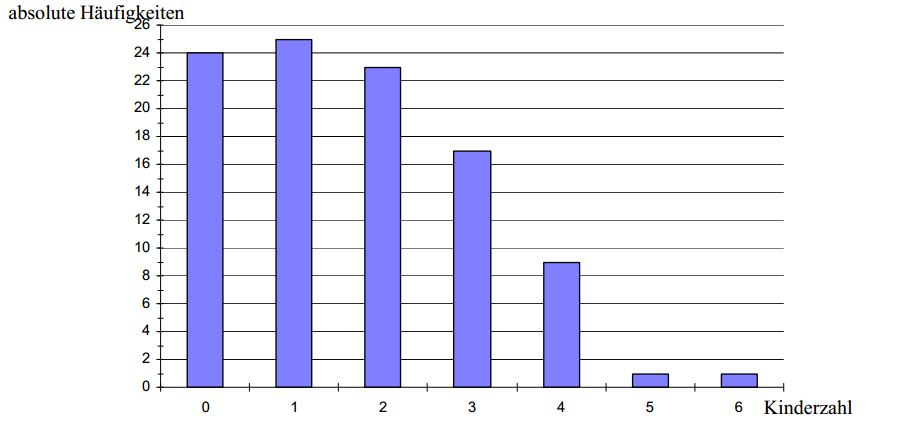
\includegraphics[width=0.9\textwidth,page=1]{./Grafiken/AB_1_8.jpg}} \caption{Erkl�rung}
\end{figure}
\end{center}
\begin{enumerate} [label=\alph*)]
\item Berechnen Sie f�r diese Verteilung das arithmetische Mittel, die Varianz, die Spannweite, den Median und den Quartilsabstand! Skizzieren Sie den zugeh�rigen Boxplot!
\item Im daneben liegenden Wohnviertel mit 100 Haushalten gibt es insgesamt 250 Kinder; die Varianz des Merkmals "Kinderzahl" betr�gt unter diesen Haushalten 3. Bestimmen Sie das arithmetische Mittel und die Varianz dieses Merkmals in der Gesamtheit aller Haushalte, wenn man die beiden Wohnviertel zusammen betrachtet!
\end{enumerate}


